\chapter{Migration process}

This chapter describes the process of migrating a web application to serverless architecture. The goal of the migration is to explore the feasibility of the catalogued patterns by applying them on common problems in the domain of web application development. In cases where the patterns prove insufficient or unsuitable to the problem in hand, modifications or new patterns are proposed. As well as exploring the patterns we're seeing how the distinct serverless features drive application design and trying to gain deeper understanding of the advantages and shortcomings of the paradigm. Finally in chapter \ref{cha:evaluation} the migration outcome is evaluated against the pre-migration application in terms of quality and ease of development.

% define migration as retaining functionality while improving quality?
% TODO better describe chapter contents: identifying problems in old implementation, picking patterns to address them

\section{Image Manager}

The migrated application, Image Manager, is a tool for managing image assets. Image Manager is adapted from a real-world application, although modified in places for the sake of illustration. Similarly to a SaaS offering such as Cloudinary, the application takes user-uploaded images, performs various forms of processing and then hosts and serves the processed images to be consumed by other applications. In case of Image Manager the processing needs are threefold: rendering a thumbnail, rendering a low quality image placeholder (LQIP), and automatic label detection. Thus in short Image Manager can be split into three basic functional requirements: image upload, image processing and image hosting.

The pre-migration serverful Image Manager consists of a single server application that connects to a number of BaaS-type cloud services, as depicted in component diagram \ref{fig:serverfulArchitecture}. The server application publishes a single HTTP API endpoint for image uploads which is consumed by a browser client. In place of access control this public-facing API uses a CAPTCHA: before image upload the client requests a challenge from Google reCAPTCHA API, solves it and sends the obtained token along with the image upload request. The server application then also connects to reCAPTCHA API to verify token validity before proceeding with the upload request. A CAPTCHA is used instead of full-blown authentication to allow for anonymous users while still providing some degree of protection against bots and other illicit usage. After CAPTCHA verification the application proceeds with image processing. The thumbnail and LQIP rendering tasks are performed locally whereas labeling is handled by a network call to an external image analysis service, Google Cloud Vision API. The three processing tasks are independent and performed concurrently. Finally both the original and processed images are uploaded to Google Cloud Storage where they can be fetched via publicly accessible URLs. Figure \ref{fig:serverfulSequence} illustrates the image upload sequence in detail, showing how the components fit together.

\begin{figure}[h]
  \centering
  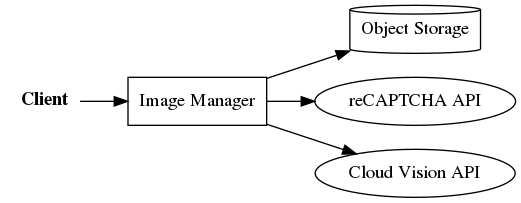
\includegraphics[width=0.65\textwidth]{image-manager.png}
  \caption{Serverful Image Manager components}
  \label{fig:serverfulArchitecture}
\end{figure}

\begin{figure}[h]
  \centering
  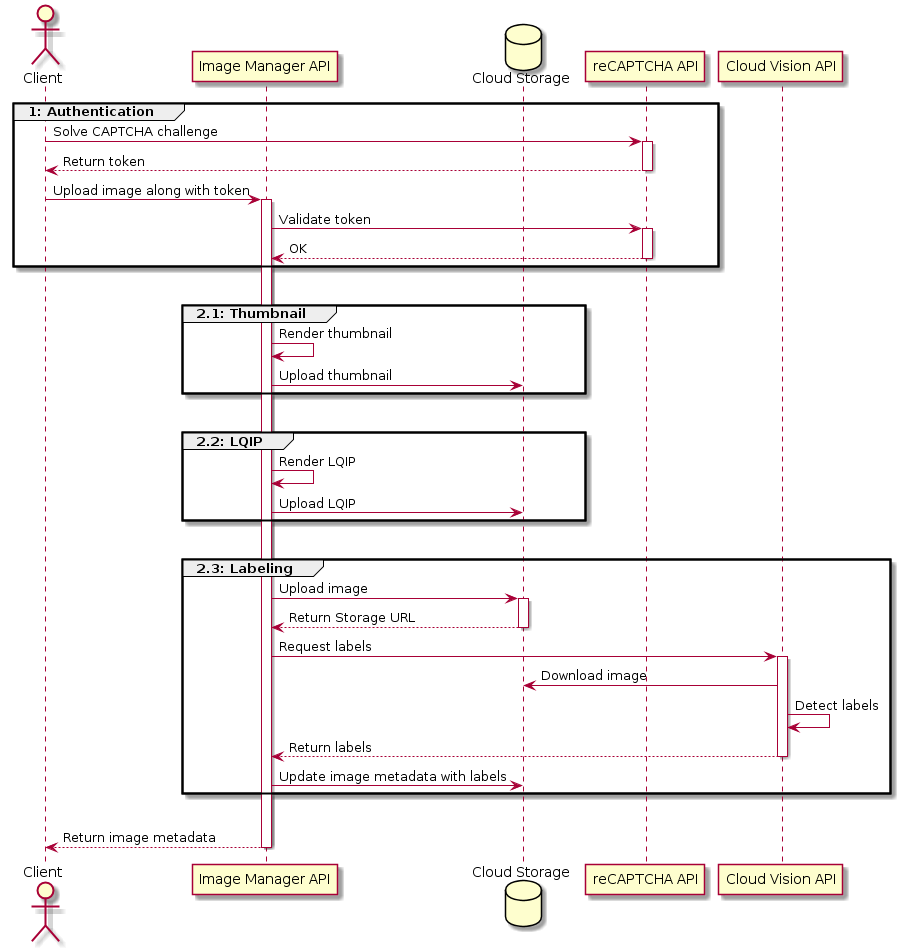
\includegraphics[width=1\textwidth]{sequence.png}
  \caption{Serverful Image Manager upload sequence}
  \label{fig:serverfulSequence}
\end{figure}

Overall the image upload task is both CPU-intensive due to local rendering and IO-heavy due to cloud service requests and also since processing results are temporarily written on disk before cloud storage upload. As for technical details, Image Manager is written in TypeScript, transpiled into JavaScript and running on NodeJS v10. The server application is containerized into a Docker image and deployed on a single VM on Google Cloud Platform's us-east1 region. The VM exposes an IP address through which the application is accessed from public internet.

Image Manager can even in its pre-migration state be considered ``cloud-ready'' in the sense that it was originally designed and developed to run specifically in a cloud environment \parencite{pozdniakova17cloudready}. This is reflected in the usage of container technology and the reliance on cloud platform services in favour of self-managed code. The degree of cloud-readiness should be kept in mind when considering the migration process as the practices and observations might not apply when starting off with a more conventional on-premise application architecture.

The motivation to migrate Image Manager to serverless architecture stems from a number of shortcomings in the current implementation, specifically relating to the non-functional requirements of availability, scalability, cost-efficiency and isolation. First, the obvious drawback of the server application's single-VM deployment is poor availability as there is no failover instance to take over in case of VM failure. Likewise the application's capacity to serve traffic is limited by a single VM's computing resources as there is no scaling mechanism in play. Achieving this double goal of availability and scalability, i.e. ensuring a correct number of VMs to meet current demand at all times would require a considerable amount of infrastructure configuration involving load balancing, clusterization and scaling policies \parencite{jonas19berkeleyView}. This inelasticity also results in cost-inefficiency as the VM instance is constantly running and accumulating charges whether or not there's any traffic. Lack of isolation is also a major concern, primarily since all application logic including image processing tasks are bundled together into a single monolithic application. This causes resource contention, as for example high CPU usage in one of the rendering tasks can divert resources from the API and result in connection timeouts. This combined with processing tasks' highly asymmetrical performance profiles also further complicates scaling as we can only scale the whole application, not just the bottlenecks. Lack of isolation also presents itself in how all traffic is routed through the server application, which in case of image uploads means an extra network trip before reaching Cloud Storage. Finally, the server application's monolithic design has negative maintainability implications since modifications cannot be developed or deployed independently.

\section{Serverless Image Manager}

Rewriting an application in serverless architecture is clearly not a trivial task nor does it have a single correct solution. Comparable to building a system out of microservices or plotting class hierarchy in object-oriented software design, the same outcome can be achieved with a variety of different but equally valid compositions of FaaS and BaaS components. As a baseline the serverless Image Manager should fulfill the same functional requirements as its predecessor. Building on that the migration should improve the application's quality attributes, particularly concerning the deficiencies listed above.

Looking at Image Manager's components in figure \ref{fig:serverfulArchitecture}, it's notable that the system's non-functional deficiencies stem from the server application and not from the integrated cloud services. The services are fully provider-managed, scale to demand and follow a pay-per-use pricing model: they don't constitute an operational overhead nor limit the application's elasticity scaling- or pricing-wise. A serverless Image Manager can therefore retain these integrations while reimplementing the server application in FaaS. While the services themselves remain the same, what changes is the way they're interfaced with since a FaaS consumer can necessitate different communication patterns than a conventional one: publish-subscribe instead of request-response, for example. As for the server application, it has two main responsibilities: first, it acts as a glue component that binds together BaaS components. Second, it provides the kind of custom server-side functionality that we cannot or choose not to offload to external services, namely thumbnail and LQIP rendering. Seeing how these responsibilities match identically with the role of FaaS in serverless systems as discussed in section \ref{sec:faasbaas}, we can expect FaaS to provide a fitting serverless alternative and migration target for the server application.

The simplest FaaS implementation of Image Manager involves wrapping the whole server application into a single function that is then invoked synchronously via HTTP. This arrangement is from the client's point of view identical to the container deployment since the function's exposed HTTP trigger acts just like the server application's HTTP API. It also already manages to shift a majority of operational concerns on to the provider. However in many cases this approach is limited by the platform's restrictions on function size and computing resources. A single monolithic function also does little to improve isolation and maintainability. If allowed by platform limits the approach can nonetheless be a good starting point for a migration: akin to the Strangler pattern (\ref{subsec:strangler}) first migrate the application into a single function and then incrementally split it off into smaller units.

\subsection{Pattern selection}

Taking full advantage of the FaaS platform's capabilities requires a more thorough redesign than simply packaging an application as-is into a single function. The design process used here is based on the pattern catalogue of chapter \ref{cha:patterns}. First each pattern is evaluated against the migrated application's functional and non-functional requirements. The patterns that most closely work towards meeting these requirements are then selected, and the selected patterns are finally composed together to form the proposed serverless design. Applying the process to Image Manager resulted in the following set of patterns: Event Processor, Fan-out/Fan-in, Thick Client, Valet Key and Bulkhead.

First of all the requirement for cost-efficiency leads towards the Event Processor pattern (\ref{subsec:Eventprocessing}). The image processing tasks should be event-driven: executed on-demand whenever there are images to process and not consume any resources or amass charges otherwise. Technically this is implemented by splitting image processing into a new function that subscribes to Cloud Storage upload events so that each image upload triggers a function invocation. The pattern also improves scalability since a large number of uploads results in a similarly large number of function invocations.

A further improvement on scalability is gained with the Fan-out/Fan-in pattern (\ref{subsec:FanoutFanin}) by splitting the three separate image processing tasks into their own functions. As each upload now triggers not one but three parallel functions, CPU-intensive rendering tasks can scale independently from the less intensive labeling task. We also observe a performance benefit as the overall task is completed faster.

With the Event Processor there's no longer a need for an API layer that receives uploads and initiates processing. Instead we can apply the Thick Client pattern (\ref{subsec:thickClient}) and have clients connect directly to Cloud Storage. This connection is secured using the Valet Key pattern (\ref{fig:valetKey}) which involves signing temporary authorization tokens for service access. The Bulkhead pattern (\ref{subsec:Bulkhead}) is used in turn to implement the Valet Key: the authorizer code is split off into its own function to ensure access to Cloud Storage even when other parts of the system are under high load.

% TODO Function Warmer for authorizer?

Figure \ref{fig:serverlessArchitecture} presents the migrated serverless architecture. The old functionality is split into four different functions and tied together in an event-driven flow. Figure \ref{fig:serverlessSequence} illustrates the image upload sequence.

serverless Image Manager doesn't expose any API apart from the authenticator; connect directly to Cloud Storage via their SDK/REST API.

% TODO Building both deployment artifacts from the same code base. describe migration process step-by-step? API, authentication, processing and upload?

\begin{figure}[h]
  \centering
  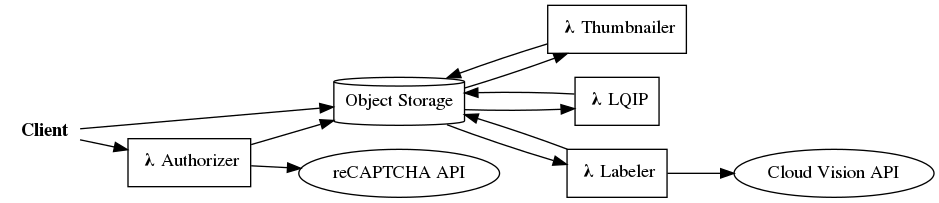
\includegraphics[width=\textwidth]{image-manager-serverless.png}
  \caption{Serverless Image Manager architecture}
  \label{fig:serverlessArchitecture}
\end{figure}

\begin{figure}[h]
  \centering
  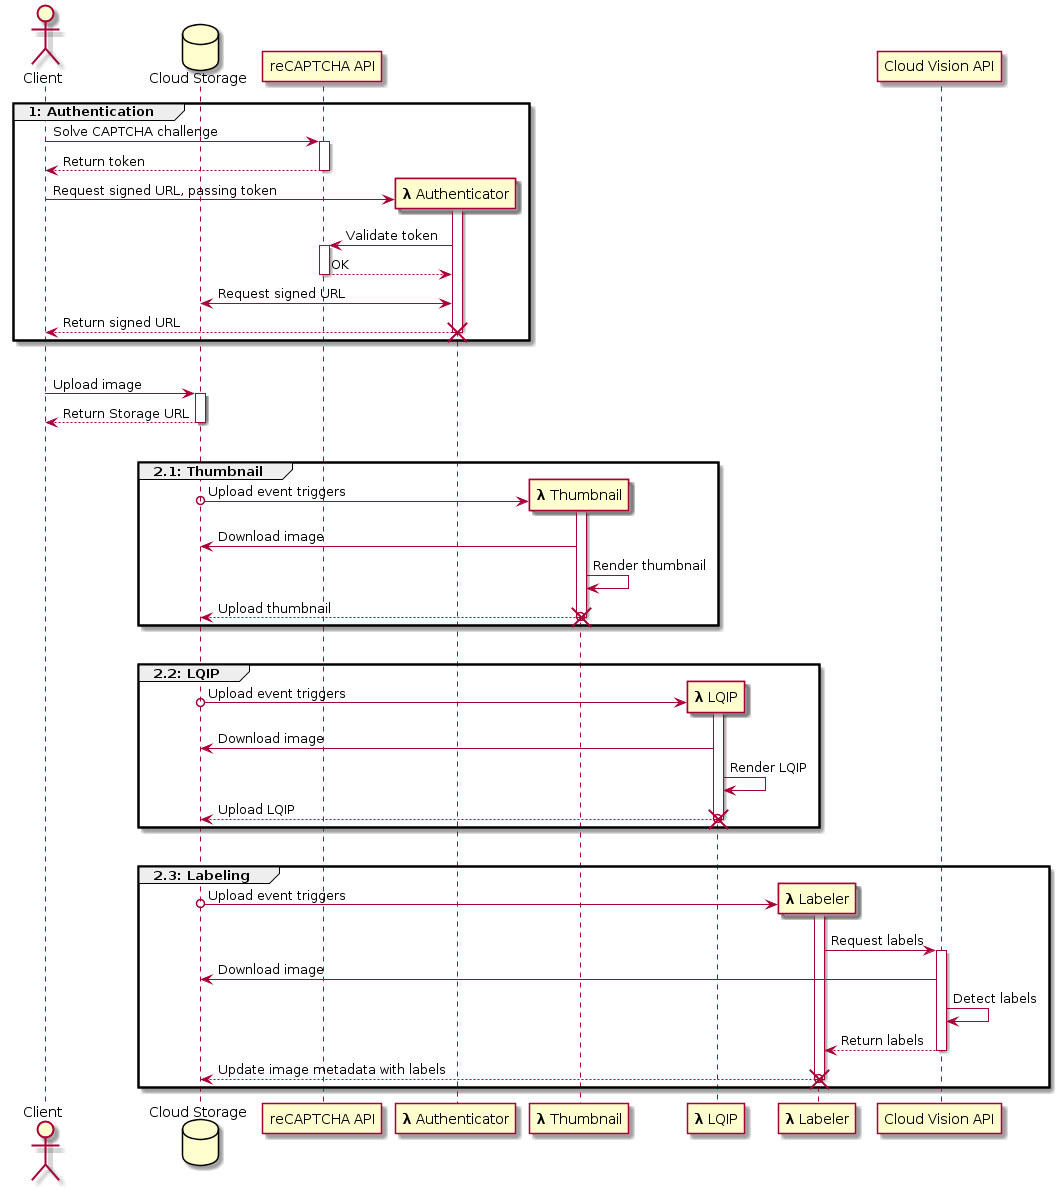
\includegraphics[width=1\textwidth]{sequence-serverless.png}
  \caption{Serverless Image Manager upload sequence}
  \label{fig:serverlessSequence}
\end{figure}

\begin{lstlisting}[language=JavaScript,caption=Image labeler function handler,captionpos=b,label=lst:labelerhandler,showstringspaces=false,belowskip=2em,frame=tb,aboveskip=2em]
  import { Storage } from '@google-cloud/storage'
  import { getBucketFileLabels } from '../label'

  const gcs = new Storage()

  export async function labeler(data) {
    const labels = await getBucketFileLabels(data)

    return gcs
      .bucket(data.bucket)
      .file(data.name)
      .setMetadata({ metadata: { Labels: labels } })
  }
\end{lstlisting}

\section{New patterns} \label{sec:newPatterns}

% TODO move to the end of Evaluation chapter?
Here are some patterns to address problems I came across while sketching out the above serverless implementation:

\subsection{Fetcher} \label{subsec:Fetcher}
% or Local Threader?

\textbf{Problem:} Scaling an IO-bound operation out to parallel function instances is inefficient since the instances compete of the same IO resources.

\textbf{Solution:} Use local threading inside a single function instance to efficiently scale out operations like network requests.

E.g. three parallel functions each making a network request, or three parallel functions invoked by cloud storage upload that start execution by downloading the image: is it more efficient to have one function download the image and then invoke/pass the image as argument to three processing functions?

\subsection{Asynchronous Response} \label{subsec:AsyncResponse}

\textbf{Problem:} The client doesn't get any feedback from the asynchronous tasks it triggers.

\textbf{Solution:} Use a pub/sub channel to send a message to the client at the end of the task.

\subsection{Task Manager} \label{subsec:taskManager}

\textbf{Problem:} The client, after triggering an asynchronous task, has no way of tracking task progress or cancelling it.

\textbf{Solution:} Make each function instance subscribe to a pub/sub channel in the beginning of its execution in order to listen to client commands.

The former is one-way pub/sub, in Task Manager the function also subscribes.

\subsection{Throttled Recursion} \label{subsec:throttledRecursion}

\textbf{Problem:} Recursive serverless functions can overwhelm downstream resources by scaling out quickly or result in an infinite loop.

\textbf{Solution:} Pass recursive invocations through a message queue in order to control recursion speed.
